\documentclass[12pt]{article}
%\documentclass[border=0.1cm]{standalone}
\usepackage{wasysym}
\usepackage{phonenumbers}
\usepackage{marvosym }
\usepackage{xcolor}
\usepackage{comment}
\usepackage{pdfpages}
\usepackage[super]{nth}
\usepackage[paperwidth=8.5in,paperheight=11in,margin=0.5in]{geometry} 
\usepackage[UKenglish]{babel}
\usepackage[UKenglish]{isodate}% http://ctan.org/pkg/isodate
\usepackage{hyperref}
\hypersetup{
  colorlinks   = true, %Colours links instead of ugly boxes
  urlcolor     = black, %Colour for external hyperlinks
  linkcolor    = black, %Colour of internal links
  citecolor   = black %Colour of citations
}
\usepackage[final]{microtype}
\frenchspacing
\usepackage[nodayofweek,level]{datetime}
\usepackage{calc,url}
\newcounter{qz}\setcounter{qz}{0}
\newcommand{\qz}{%\
\setcounter{qz}{\value{qz}+1}
\textbf{In-class  \theqz} \,}

\newcounter{hw}\setcounter{hw}{0}
\newcommand{\hw}{%\
\setcounter{hw}{\value{hw}+1}
\textbf{HW \thehw}}

\makeatletter
\newcommand*{\rom}[1]{\expandafter\@slowromancap\romannumeral #1@}
\makeatother

\newcounter{ex}\setcounter{ex}{0}
\newcommand{\ex}{%\
\setcounter{ex}{\value{ex}+1}
Exam \rom{\theex}}

\usepackage[T1]{fontenc} 
\usepackage{fourier}
%\usepackage{tgschola} %to look retro
\newenvironment{mypar}[2]
  {\begin{list}{}%
    {\setlength\leftmargin{#1}
    \setlength\rightmargin{#2}}
    \item[]}
  {\end{list}}


\newcounter{wk}\setcounter{wk}{0}
\newcommand{\wk}{%\
\setcounter{wk}{\value{wk}+1}
\thewk \,\,}

\usepackage[nomessages]{fp}% http://ctan.org/pkg/fp


\usepackage{enumerate}
\usepackage{graphicx}
\usepackage{fontawesome}
\newcommand{\cvgithub}[1]{\renewcommand{\cvgithub}{#1}}
\usepackage{paralist}
\renewenvironment{description}[0]{\begin{compactdesc}}{\end{compactdesc}}

\newenvironment{alphalist}{
  \begin{enumerate}[(a)]
    \addtolength{\itemsep}{-0.5\itemsep}}
  {\end{enumerate}}
  \cleanlookdateon% Remove ordinal day reference
  \newcommand{\RomanNumeralCaps}[1]
      {\MakeUppercase{\romannumeral #1}}

\usepackage{xspace}
\makeatletter
\DeclareRobustCommand{\maybefakesc}[1]{%
  \ifnum\pdfstrcmp{\f@series}{\bfdefault}=\z@
    {\fontsize{\dimexpr0.8\dimexpr\f@size pt\relax}{0}\selectfont\uppercase{#1}}%
  \else
    \textsc{#1}%
  \fi
}
\newcommand\AM{\,\maybefakesc{am}\xspace}
\newcommand\PM{\,\maybefakesc{pm}\xspace}
\makeatother

 \newcommand{\coursename}{Numerical Analysis \\ Foundations of Computational Mathematics }
\newcommand{\coursenumber}{MATH 420--01 and CYBR 304--01}
\newcommand{\sectionnumber}{}
\newcommand{\term}{Spring }
\newcommand{\room}{Discovery Hall, room  116}
\newcommand{\meetingtime}{This class meets Monday, Wednesday, and Friday  from 
	8:00\AM -- 8:50\AM}
\newcommand{\officehours}{ Monday, Wednesday, and Friday 9:00\AM---11:00\AM,
    Tuesday and Thursday 9:30\AM---11:00\AM, and by appointment.}

    \newcommand{\finaldateandtime}{\printdate{13/5/\the\year} 8:00\AM{}---10:00 \AM}
\begin{document}
\cleanlookdateon% Remove ordinal day reference
\shortdate
\printyearoff
\large
\begin{center}
    \textbf{\coursename}  \\
    {\coursenumber} \\
     {\term \the\year} \\
\end{center}

\vskip0.25in
\normalsize


\begin{center}
\begin{description}
    \item[Instructor:] Barton Willis, PhD, Professor of Mathematics
    \item[Office:]  Discovery Hall, Room 368
    \item[Office Hours:] \officehours
   % \item[Zoom] 616 568 5706
    \item[\phone:]  \phonenumber[country=US]{3088658868}
    \item[\Email:]  \href{mailto:willisb@unk.edu}{willisb@unk.edu}
    \item[\faGithub]   \url{https://github.com/barton-willis/MATH-420-CYBR-304}

  \end{description}
\end{center}



\subsubsection*{Important Dates}

\begin{mypar}{0.25in}{0.25in} 

  \textbf{First homework due} \dotfill  \printdate{27/1/\the\year}  \\
  \textbf{Exam \rom{1}} \dotfill \printdate{23/2/\the\year}  \\
  \textbf{Exam \rom{2}} \dotfill  \printdate{5/4/\the\year} \\
  \textbf{Exam \rom{3}} \dotfill \printdate{3/5/\the\year} \\
  \textbf{Final exam} \dotfill  \finaldateandtime
\end{mypar}

\subsubsection*{Grading}

Your course grade will be based on eleven homework sets, three midterm exams, and a comprehensive 
final exam; specifically:
\FPeval{\hwpts}{round(20*11,0)}
\begin{mypar}{0.25in}{0.25in}
    \textbf{Weekly Homework:}  \emph{11 twenty point assignments}  \dotfill \hwpts\/ (total) \\
    \textbf{Mid-term exams \rom{1}, \rom{2}, \rom{3}:} \emph{100 points each} \dotfill 300 (total)\\
    \textbf{Comprehensive Final exam} \dotfill 150 (total)
\end{mypar}
If we end the term with less than \hwpts\/ points for homework,  
your homework point total will be scaled to \hwpts\/ points. 
There will be a five point bonus that is due the first week of the 
term.

\FPeval{\points}{round(11*20+300+150,0)}

\FPeval{\F}{round(\points*0.6-1,0)}
\FPeval{\Dm}{round(\points*0.6,0)}
\FPeval{\D}{round(\points*0.633,0)}
\FPeval{\Dp}{round(\points*0.6666667,0)}

\FPeval{\Cm}{round(\points*0.7,0)}
\FPeval{\C}{round(\points*0.733,0)}
\FPeval{\Cp}{round(\points*0.7666667,0)}

\FPeval{\Bm}{round(\points*0.8,0)}
\FPeval{\B}{round(\points*0.833,0)}
\FPeval{\Bp}{round(\points*0.8666667,0)}

\FPeval{\Am}{round(\points*0.9,0)}
\FPeval{\A}{round(\points*0.933,0)}
\FPeval{\Ap}{round(\points*0.99,0)}

The following table shows the \emph{minimum} number of points (out of \points) that
are required for each of the twelve letter grades D- through A+. For
example, a point total of \Bp\/  points will earn you a grade of B+,  and 
a point total of \Am\/ points will earn you a grade of A-. If you earn a point
total of \F\/  or less, you will a failing course grade.
  \begin{center}
     \begin{minipage}{5.5in}
\begin{mypar}{0.25in}{0.25in}
    \begin{minipage}{2.5in}
        D-  \dotfill \Dm \\
        D \dotfill \D \\
        D+ \dotfill \Dp \\
        C- \dotfill \Cm  \\
        C \dotfill \C \\
        C+ \dotfill \Cp 
        \end{minipage}
    \phantom{xxxxx}
    \begin{minipage}{2.5in}
        B- \dotfill \Bm \\
        B \dotfill  \B \\
        B+ \dotfill  \Bp\\
        A- \dotfill  \Am \\
        A \dotfill  \A \\
        A+ \dotfill  \Ap
    \end{minipage}
\end{mypar} 
\end{minipage}
\end{center}

\subsubsection*{Course Calendar}

We will try to adhere to the following schedule, but we will modify it
if needed. The exam dates will only be changed for a compelling
reason; we won't delay an exam because we are behind the
schedule. Neither will an exam date be moved forward because we are
ahead of the schedule.

Homework assignments are due at 11:59 \PM local time on Saturday on the week they are assigned. 

\vspace{0.1in}

\begin{center}

\begin{tabular}  {|l|l|l|l|l|}
\hline
{\bf Week}  & {\bf Week} &  {\bf Section(s)} & {\bf Topic(s)} & {\bf Assessment} \\
\hline \hline 
\wk    & 1/22 & \S1.1, \S1.3      &  Floating point numbers \& calculus tools  &  \hw  \\
\wk    & 1/29 &    \S1.2   &   Introduction to Julia  & \hw \\
\wk    & 2/5 &    \S2.1 & Errors and convergence rates    & \hw \\
\wk    & 2/12  & \S2.2 -- \S2.7 &  Root Finding   &  \hw \\
\wk    & 2/19 &  \S2.2--\S2.7   &  Root Finding    &  \textbf{\ex, 23 Feb}   \\
\wk    & 2/26 &  class notes                    &    Linear equations                    &    \hw                                  \\
\wk    & 3/4   &  class notes     &  Linear equations  &   \hw    \\
\wk    & 3/18     & \S3.1--\S3.4 & Interpolation &  \hw   \\
\wk   & 3/25   & \S3.1 -- \S3.4   &   Interpolation   & \hw \\
\wk  &  4/1   & \S4.1--\S4.2 &  Numerical  integration  & \textbf{\ex , 5 April}  \\
\wk &  4/8    &   \S4.3 --\S4.4 &   Gaussian integration \& multiple integrals   &  \hw  \\
\wk  & 4/15 &   \S5.1--\S5.2 & Discrete \& continuous least squares  &  \hw  \\
\wk   & 4/22  & \S5.3 &  Orthogonal polynomials and least squares  & \hw  \\
\wk   & 4/29   &   class notes      & Differential equations &  \textbf{\ex, 3 May}     \\
\wk   & 5/6   &  class notes       & Differential equations   &  \\
\wk   & 5/13       &  &  &  \textbf{Final 13 May,  8:00 am--10:00 am} \\ \hline
\end{tabular}
\end{center}

\subsubsection*{Class meeting time and place}

\meetingtime in \room.


\subsubsection*{Course Objectives}

On completion of this course, students will
\begin{alphalist}
    \item understand IEEE arithmetic and know the rules for accurate computation.
    \item understand the concepts of linear and quadratic convergence and use these concepts to analyze 
        the efficiency of an algorithm.
    \item develop an understanding of the algorithms for solving linear and nonlinear equations, interpolation, 
       quadrature, least squares methods, and solution of differential equations.
    \item be able to use a programming language and graphical tools to solve problems numerically.
\end{alphalist}
 

\subsubsection*{Course Resources}

\begin{enumerate}

\item Our textbook is \emph{First Semester in Numerical Analysis with Julia,} by Giray Ökten.  This is an open-source textbook that can be legally downloaded, printed, and  used without payment.\footnote{\tiny
\url{https://diginole.lib.fsu.edu/islandora/object/fsu:657877/datastream/PDF/view} \normalsize} For topics not covered in our textbook, we'll use class notes and other freely available resources.

\item Class notes that are written on the board or distributed via Canvas.

\item Reliable Internet access.

\item  An Internet connected computer (not just a phone or tablet) that can run the Juila Language.  Both are free resources; download and install Julia it from \url{https://julialang.org/downloads/}.  I suggest that you install version 1.10.0.


\item Pencils, erasers, notebook for note taking. Colored pens or pencils are nice for note taking.


 \end{enumerate}




\subsubsection* {Class Policies}

Unless an assessment is \emph{explicitly} stated to be a group project,  \emph{all work you turn in for a grade must be your own.}  If you need assistance in completing a homework assignment, you may ask me for help. Using solution keys from previous terms (either from UNK or other universities) is prohibited.  Violation of these rules will result in earning a grade of zero on the assessment. Each homework assignment you turn in for a grade must include the statement:

\begin{quote}
\fbox{I have neither given nor received unauthorized assistance on this assignment.}
\end{quote}
 If two assignments are so similar that only collaboration could explain their similarities, both assignments will receive a grade of zero.  Using unauthorized materials or communication devices (cell phone, for
example) while taking a test will earn you a grade of zero on that assessment.  

 

\begin{enumerate}

\item Regular in person class attendance is required. If you are ill or need to miss a 
class due to athletics, please let me know ahead of time and I will make an effort to put the class on Zoom. Additionally,
when you miss class, please ask a classmate to take class notes for you.  My class notes are intended for my use and they are \emph{not} a good guide to our class, so generally I will not provide you with my class notes. 

\item For examinations and in class assignments, show your work.  \emph{No credit will be given for multi-step problems without the necessary work. Your solution must contain enough detail
so that I am convinced that you could correctly work any similar problem.} Also erase or clearly mark any work you want me to ignore; otherwise,
I'll grade it.  

\item The work you turn in is expected to be \emph{accurate, 
complete, concise, neat}, and \emph{well-organized}.  
\emph{You will not earn full credit on work that falls short of 
these expectations.}

\item Class cancellations due to weather, illness, or other 
unplanned circumstances may require that we make  adjustments
to the course calendar, exam dates, and due dates or specifics for 
course assessments. 


\item Extra credit is not allowed. Redoing an assessment to earn a higher grade is not allowed.

\item I will accept homework that is submitted late only with prior approval and for a good and substantial reason. Homework 
that is submitted late with no prior approval will not be graded and will earn you a grade of zero.

\item For examinations, you may use a teacher provided quick reference sheet (if any)
but no other reference materials.  You may also use a pencil, eraser, 
and a scientific calculator. For examinations, your phone and all such
devices must be turned off and \emph{out of sight}. 

\item Generally, if you are ill or absent for any reason (including 
athletics), you must turn in your in class work on time. Permission to
turn in work late must be made in advance, otherwise late in class work 
will count zero points.


 

\item During class time, please refrain from using electronic devices. If your 
device usage distracts your classmates, I will ask you to put it away. If it's my 
impression that you are often not paying attention in class, I reserve the right to 
decline to help you during office hours.

\item The final examination will be \emph{comprehensive} and it will be given 
during the  time scheduled by the University. Except for \emph{extraordinary circumstances}
you must take the exam at this time.
 
\item If you have questions about how your work has been graded, make an appointment with me immediately.


\item Please regularly check Canvas  to verify that your scores have 
been recorded correctly.  If I made a mistake in recording one of
your grades, I'll correct it provided you saved your paper.



\end{enumerate}

















\newpage



\subsubsection*{University Policies\footnote{These polices are
copied from \url{https://catalog.unk.edu/undergraduate/academics/academic-regulations/}
and from \url{https://www.unk.edu/academic_affairs/asa_forms/course-policies-and-resources.php}.
As of 29 May \the\year, these polices are current.}} 
\paragraph*{Student Attendance Policy Statement}

Students are expected to attend all meetings of classes for which they are 
registered, including the first and last scheduled meetings and the final 
examination period. Instructors hold the right and responsibility to 
establish attendance policies for their courses. Each instructor must 
inform all classes at the beginning of each semester concerning their 
attendance policies.

Participation in official University activities, serious health concerns, 
personal emergencies, and religious observances are valid reasons for absence 
from classes. Students are responsible for informing their instructors prior 
to their absence(s) from class and for completing assignments missed during 
their absence(s). No adverse or prejudicial effects shall result to any student 
with a documented, excused absence.  

Questions may be directed to the Dean of Student Affairs office or to Student 
Health \& Counseling.


\paragraph{Academic Integrity Policy}

The maintenance of academic honesty and integrity is a vital concern 
of the University community. Any student found in violation of the 
standards of academic integrity may be subject to both academic and 
disciplinary sanctions. Academic dishonesty includes, but is not 
limited to, the following:

\begin{itemize}
    \item \textbf{Cheating} Copying or attempting to copy from an academic 
    test or examination of another student; using or attempting to 
    use unauthorized materials, information, notes, study aids or 
    other devices for an academic test, examination or exercise; 
    engaging or attempting to engage the assistance of another 
    individual in misrepresenting the academic performance of a 
    student; or communicating information in an unauthorized manner 
    to another person for an academic test, examination or exercise.
    
    \item \textbf{Fabrication and falsification} Falsifying or 
    fabricating any information or citation in any academic exercise, 
    work, speech, test or examination. Falsification is the 
    alteration of information, while fabrication is the invention 
    or counterfeiting of information.

    \item \textbf{Plagiarism}  Presenting the work of another as one's 
    own (i.e., without proper acknowledgment of the source) and 
    submitting examinations, theses, reports, speeches, drawings, 
    laboratory notes or other academic work in whole or in part as 
    one's own when such work has been prepared by another person or 
    copied from another person.

    \item \textbf{Abuse of academic materials and/or equipment} 
    Destroying, defacing, stealing, or making inaccessible library 
    or other academic resource material.

    \item \textbf{Complicity in academic dishonesty} Helping or 
    attempting to help another student to commit an act of academic 
    dishonesty.

    \item \textbf{Falsifying grade reports} Changing or destroying 
    grades, scores or markings on an examination or in an 
    instructor's records.

    \item \textbf{Misrepresentation to avoid academic work} 
    Misrepresentation by fabricating an otherwise justifiable 
    excuse such as illness, injury, accident, etc., in order 
    to avoid or delay timely submission of academic work or to 
    avoid or delay the taking of a test or examination.
    
    \item \textbf{Other Acts of Academic Dishonesty} Academic units 
    and members of the faculty may prescribe and give students prior 
    written notice of additional standards of conduct for academic 
    honesty in a particular course, and violation of any such 
    standard shall constitute a violation of the Code.

\end{itemize}
Under Section 2.9 of the Bylaws of the Board of Regents of the 
University of Nebraska, the respective colleges of the University 
have responsibility for addressing student conduct solely affecting 
the college. Just as the task of inculcating values of academic 
honesty resides with the faculty, the college faculty 
are entrusted with the discretionary authority to decide 
how incidents of academic dishonesty are to be resolved. 
For more information, please visit UNK's Procedures and 
Sanctions for Academic Integrity and the Student Code of Conduct.


\paragraph{Reporting Student Sexual Harassment, Sexual Violence or Sexual Assault}

Reporting allegations of rape, domestic violence, dating violence, sexual assault, 
sexual harassment, and stalking enables the University to promptly provide support 
to the impacted student(s), and to take appropriate action to prevent a recurrence 
of such sexual misconduct and protect the campus community. Confidentiality will 
be respected to the greatest degree possible. Any student who believes they may 
be the victim of sexual misconduct is encouraged to report to one or more of 
the following resources:

\begin{itemize}
\setlength\itemsep{-0.25em}
  \item Local Domestic Violence, Sexual Assault Advocacy Agency 
      \phonenumber[country=US]{3082372599}

  \item Campus Police (or Security) \phonenumber[country=US]{3088658911}

  \item Title IX Coordinator \phonenumber[country=US]{3088658655}
\end{itemize}
Retaliation against the student making the report, whether by students or 
University employees, will not be tolerated.

\paragraph{Students with Disabilities} It is the policy of the University of Nebraska 
at Kearney to provide flexible and individualized reasonable accommodation 
to students with documented disabilities. To receive accommodation services 
for a disability, students must be registered with the UNK Disabilities Services 
for Students (DSS) office, 175 Memorial Student Affairs Building, 
\phonenumber[country=US]{3088658214} or by email 
\href{mailto:unkdso@unk.edu}{unkdso@unk.edu}  


\paragraph{Students Who are Pregnant} It is the policy of the University of Nebraska at Kearney to provide flexible and 
individualized reasonable accommodation to students who are pregnant. To receive 
accommodation services due to pregnancy, students must contact the 
Student Health office at \phonenumber[country=US]{3088658218}. The following links provide information 
for students and faculty regarding pregnancy rights: 

\begin{itemize}
\setlength\itemsep{-0.25em}
\item \url{https://thepregnantscholar.org/title-ix-basics/} 

\item \url{https://nwlc.org/resource/faq-pregnant-and-parenting-college-graduate-students-rights/}

\end{itemize}

\paragraph{UNK Statement of Diversity \& Inclusion}

UNK stands in solidarity and unity with our students of color, our Latinx 
and international students, our LGBTQIA+ students and students from other 
marginalized groups in opposition to racism and prejudice in any form, 
wherever it may exist. It is the job of institutions of higher education, 
indeed their duty, to provide a haven for the safe and meaningful exchange of 
ideas and to support peaceful disagreement and discussion. In our classes, 
we strive to maintain a positive learning environment based upon open 
communication and mutual respect. UNK does not discriminate on the basis of 
race, color, national origin, age, religion, sex, gender, sexual orientation, 
disability or political affiliation. Respect for the diversity of our backgrounds 
and varied life experiences is essential to learning from our similarities as 
well as our differences. The following link provides resources and other 
information regarding D\&I: \url{https://www.unk.edu/about/equity-access-diversity.php}.

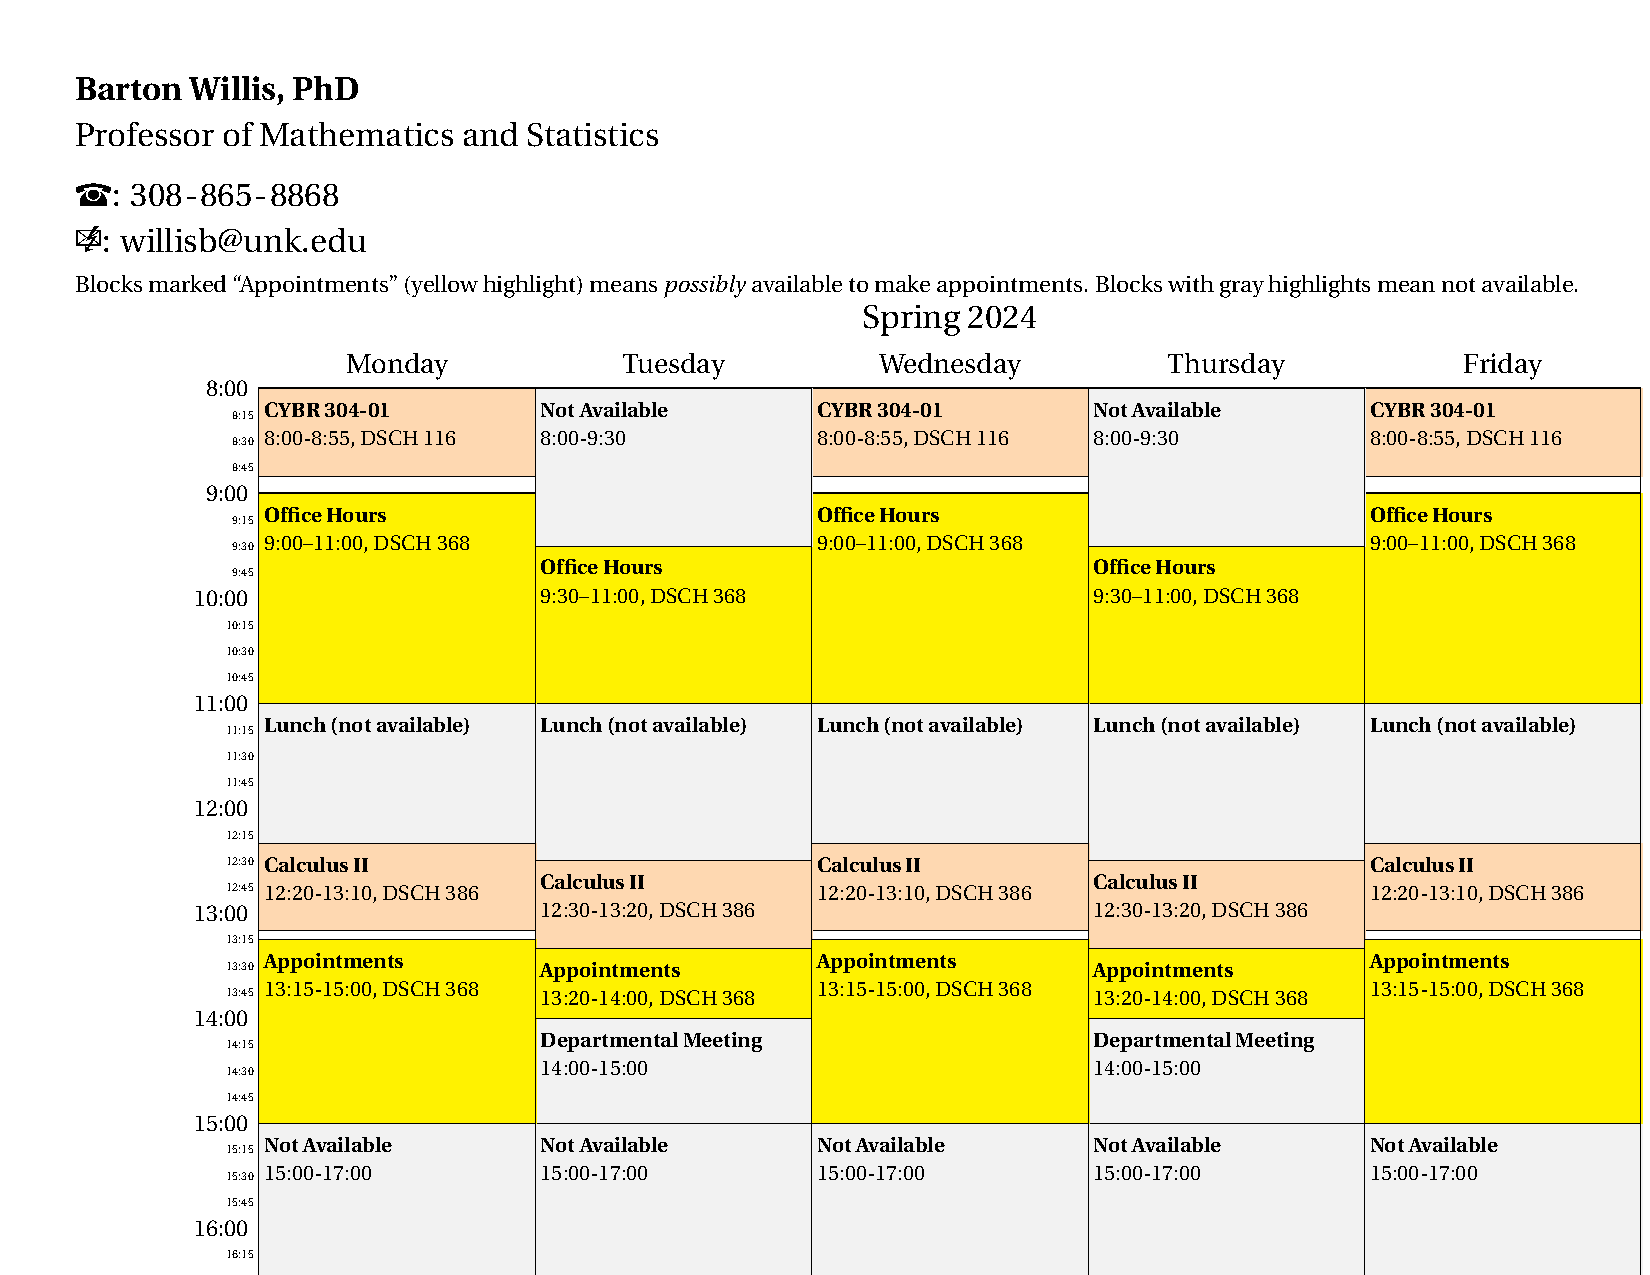
\includepdf[pages={1-},angle=90]{door_schedule.pdf}  
\end{document}

\vspace{0.1in}

\begin{center}

\begin{tabular}  {|l|r|l|l|}
\hline
{\bf Week}  & {\bf Week of} & {\bf Month}&  {\bf Topic(s)} \\
\hline \hline
\wk    & 12 & Jan  & algorithms and an introduction to Maxima (classnotes) \\\
\wk    & 19 &     &  IEEE arithmetic and the condition number (Chapter 0) \\
3    & 26 &     & interval arithmetic and running errors (classnotes) \\
4    & \phantom{1}2 & Feb   &  solving equations, Chapter 1 \\
5    & 9  &  & solving equations, Chapter 1; \textbf{Exam 1, 13 Feb.} \\
6    & 16 & & numerical linear algebra, Chapter 2 \\
7    & 23 &  & numerical linear algebra, Chapter 2 \\
8    & \phantom{1}2 & Mar  & interpolation and least squares, Chapters 3 and 4 \\
9    & 9 &    & numerical differentiation and integration, Chapter 5; \textbf{Exam 2, 13 March} \\
10    & 23 &      & numerical differentiation and integration, Chapter 5 \\
11   & 30 &     & initial value problems, Chapter 6 \\
12   & 6  & April   &   initial value problems, Chapter 6 \\  
13   & 13 &        & partial differential equations, Chapter 8 \\
14   & 20 &     & partial differential equations, Chapter 8; \textbf{Exam 3, 24 April} \\
15   & 27 &     & Fourier series  (classnotes) \\ \hline
     &      &     & \textbf{Final Exam, Wednesday 6 May, 10:30--12:30} \\ \hline
\end{tabular}
\end{center}


\end{document}

\begin{tabular}  {|l|l|l|l|}
\hline
{\bf Week}  & {\bf Week of} & {\bf Month}&  {\bf Topic(s)} \\
\hline \hline
1    & \phantom{1}9 &Jan  & Introduction \\
2    & 16 &   & Floating point numbers \\
3    & 23 &  & Condition number \& relative difference \\
4    & 30 &  & Floating point arithmetic \\
5    & \phantom{1}6 &Feb & Sums \& hypergeometic functions; \textbf{Exam 1, Friday, 11 Feb.} \\
6    & 13 &    & Linear algebra \\
7    & 20 &     & Matrix norms and condition numbers \\
8    & 27 &     & LU factorization \\
9    & \phantom{1}6 & Mar      & Eigenvalues \\
10   & 20 &    & Least squares; \textbf{Exam 2, Friday, 25 March} \\
11   &   27   &  & Interpolation \& approximation \\
12   &   \phantom{1}3 & April   & Nonlinear equations \\
13   &   10 &     &  Numerical Integration \\
14   &   17 &     & Finite differences; \textbf{Exam 3, Friday, 22 April} \\
15   &   24 &     & Partial Differential Equations \\ \hline
     &      &     & \textbf{Final Exam, Wednesday, 3 May, 8:00--10:00} \\ \hline
\end{tabular}

3    & 24  & \S2.3---\S2.4  & Norms and condition numbers \\
4    & 31  & \S3.1---\S3.3  & Least squares \\
5    & 7 Feb & \S4.1           & Eigenvalues; {\bf Exam 1, Friday, 10 Feb}\\ \hline
6    & 14 Feb & \S4.2           & Eigenvalues  \\
7    & 21 & \S5.1---\S5.2  & Nonlinear equations \\
8    & 28  & \S7.1---\S7.2  & Interpolation \& Approximation \\
9    & 7 Mar  & \S8.1---\S8.3    & Numerical integration; {\bf Exam 2, Friday, 24 March}\\
\hline
10   & 21 Mar & \S8.4           & Adaptive Integration \\
11   & 28 & \S8.7, \S9.1---\S9.2  & Finite Differences and Initial Value Problems \\
12   & 4 Apr & \S9.3---\S9.4  & Differential Equations  \\
13   & 11  & \S11.1---\S11.2 & Partial Differential Equations \\
14   & 18   & \S11.2  &   Partial Differential Equations; {\bf Exam 3, Friday. 21 April} \\
15   &  & \S12.1---\S12.3  & Fast Fourier Transform \\ \hline
16    &  & \S1.1---\S12.3    &  {\bf Final Exam Wednesday 3 May 8:00--10:00}  \\
\hline
\end{tabular}
\end{center}
\end{document}


   1.  Scientific Computing
   2. Systems of Linear Equations
   3. Linear Least Squares
   4. Eigenvalue Problems
   5. Nonlinear Equations
   6. Optimization
   7. Interpolation
   8. Numerical Integration and Differentiation
   9. Initial Value Problems for Ordinary Differential Equations
  10. Boundary Value Problems for Ordinary Differential Equations
  11. Partial Differential Equations
  12. Fast Fourier Transform
  13. Random Numbers and Stochastic Simulation 